Almost all interpretability methods work on image classification tasks. To learn how these methods are applied, how they work and what output they generate, the first step in this work is applying these methods on a classification task. We chose a dataset from the medical imaging field: The NIH (National Institutes of Health, United States) chest X-ray dataset \cite{wang2017chestx}.

We downloaded the dataset, trained a neural network on the dataset and applied the selected methods described above.

\section{NIH Chest X-ray dataset}
The NIH Chest X-ray dataset contains 112,120 X-ray scans from 30,805 unique patients \cite{nihchestxraykaggle}. Every scan has one or more disease labels. Figure \ref{chest_xray_sample} show three sample images from the dataset.

\begin{figure}[h]
\centering
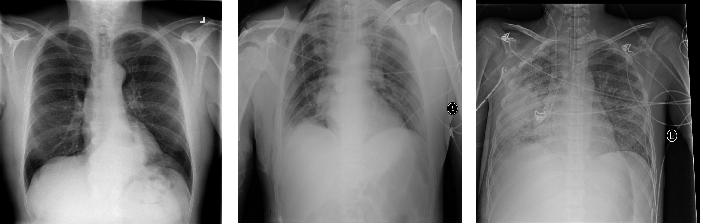
\includegraphics[width=14cm]{chapters/03_classification/images/chest-x-ray.png}
\caption{Examples for the NIH Chest X-ray dataset.}
\label{chest_xray_sample}
\end{figure}

\section{Model Training}
We decided to train a model based on an existing neural network architecture, because building a state of the art architecture is very hard and not the focus of this thesis.

The detailed results of the training sessions are available in the results directory of the GitHub repository: \href{https://github.com/andef4/thesis-code/tree/master/nhs-chest-xray/results/}{nhs-chest-xray/results}.

\subsection{Inception ResNet v2}
\nblink{nhs-chest-xray/inception\_resnetv2.ipynb}

We chose Inception ResNet v2 \cite{szegedy2017inception} as the first architecture to investigate. This is modern neural network built for image analysis.
The ResNet variant of the Inception architecture delivers similar performance as the normal Inception model, but with significantly reduced training time.

\nblink{nhs-chest-xray/preprocess.ipynb}
The preprocessing steps required to use this architecture are resizing the images to 299x299 pixels and converting the gray-scale images to color images.
We also tried to modify the network to directly use gray-scale images, but this was not successful because the network architecture is built for three channel images.

We initially trained the network on a smaller sample set (5607 image) of the dataset. The maximum reached validation accuracy was 40\%. The training times for the small training subset
were already very long, we therefore decided to abandon the Inception architecture for now and use a ResNet based architecture instead.

\subsection{ResNet}
\nblink{nhs-chest-xray/resnet.ipynb}

The first test of ResNet50 \cite{he2016deep} with pretrained parameters (trained on ImageNet) on the sample dataset showed fast training times but low accuracy. Training the network from scratch showed promising validation accuracy, which started to decrease on later epochs. As the training accuracy was still increasing, this is a clear indicator that the neural network is overfitting. We decided to change the architecture to ResNet18, which is a smaller ResNet variant with fewer parameters and should therefore be less susceptible to overfitting.

The first training run of ResNet18 with the sample dataset looked promising, so we moved to train the network on the full dataset. The results were underwhelming, with the validation accuracy maxing out at 23\%.

\subsection{Single label only}
The NIH Chest X-ray dataset is a multi class dataset. This means a single image can contain labels for multiple diseases. Training models for such datasets is much harder than training datasets where each image only has one label. We therefore decided to remove all images which contain multiple labels and only train on images with one label.

We did multiple iterations on the full dataset with ResNet18, experimenting with different parameters:
\begin{itemize}
    \item Using SGD optimizer instead of Adam
    \item Using a pretrained model vs. from scratch model
    \item Use data augmentation on the input (color jitter, random horizontal flip)
\end{itemize}

None of these parameters changed the validation accuracy significantly, always peaking around 60\% to 65\%.

\subsection{DenseNet}
\nblink{nhs-chest-xray/DenseNet.ipynb}

Researching what other people did to train a model for this dataset, we came across the CheXNet \cite{rajpurkar2017chexnet} paper and an implementation of the paper in PyTorch \cite{chexnetpytorch}.

The paper uses the DenseNet \cite{huang2017densely} architecture. An implementation of DenseNet is available in PyTorch. The implementation of the paper provided a pretrained model, but loading the saved model did not work, because the used version of PyTorch was old and incompatible with ours.

\subsection{Retraining DenseNet}
\nblink{nhs-chest-xray/DenseNet\_singleclass.ipynb}

After fixing multiple implementation errors (not correctly setting the output class count, assigning of classes to output neurons not the same in test vs. validation set), we started to get acceptable accuracy rates for the DenseNet implementation, peaking around 55\% accuracy.

\subsection{Removing "No findings" class}
The implementation of the CheXNet paper displayed an accuracy table per class. We decided to do the same for our implementation. We quickly discovered that only the "No findings" class hat correctly classified images, all other classes had zero correct classifications. The "No findings" class is by far the biggest class in the dataset. For the neural network to get a good result, the easiest way is to just declare all images to be in the class "No findings".

We removed the "No findings" class from the dataset and retrained both the ResNet18 and the DenseNet implementation, getting similar results of around 30\% accuracy.

\subsection{Weighted classes}
The dataset still has a class imbalance, even with the "No findings" class removed. To counter this problem, we calculated the percentage every class has of the full dataset and gave these information as class weight to the back propagation criterion.

This increased the accuracy to around 33\%, but should help classes which are underrepresented in the dataset.

\subsection{Conclusion}
At this point we decided to stop trying to enhance the neural network, because the training already took a long time and an accurate network is not the goal of this thesis. Some classes showed high accuracy rating, analyzing these classes should provide enough insight how the interpretability methods works.